\documentclass{article}
\usepackage{amsmath}
\usepackage{graphicx}
\usepackage{float}
\usepackage{fancyhdr}
\usepackage[spanish]{babel}
\usepackage[utf8]{inputenc}
\usepackage[justification=centering]{caption}
\usepackage[font={small}]{caption}

\setlength{\headheight}{15pt}
\parindent 0em
\parskip 2ex
\pagestyle{fancy}
\setlength{\textfloatsep}{5pt}

\newcommand{\forceindent}{\leavevmode{\parindent=1em\indent}}


\begin{document}

\begin{titlepage}
\newcommand{\HRule}{\rule{\linewidth}{0.5mm}}

\center
\textsc{\LARGE ITESO, Universidad Jesuita De Guadalajara}\\[2cm]
\textsc{\Large INGENIERÍA FINANCIERA}\\[1cm]
\textsc{\large Innovación y Gestión De Proyectos}\\[1cm]
\HRule \\[2cm]
{ \huge \bfseries Accidentes viales en la Zona Metropolitana de Guadalajara}\\[2cm]
\HRule \\[2cm]
\begin{minipage}{0.4\textwidth}
\begin{flushleft} \large


\emph{Autores:}\\
\small Alicia Karime González Beltrán\\
\small Ana Goretti Chávez Flores\\
\small Rodrigo Hernández Mota\\
\small José Felipe Sánchez Andaluz
\end{flushleft}
\end{minipage}
~
\begin{minipage}{0.4\textwidth}
\begin{flushright} \large
\emph{Supervisor:} \\
\small Mtra. Mireya \textsc{Pasillas Torres}
\end{flushright}
\end{minipage}\\[2cm]

{\large \today}\\[1cm]

\vfill
 
\end{titlepage}
\tableofcontents
\newpage

\section{Introducción}\label{sec:into}
[agregar contenido]

\newpage
\section{Diagnóstico}\label{sec:diagnostic}

Datos provenientes de la Secretaría de Movilidad de Jalisco (SEMOV) señalan que en 2016 se generaron
más de \textbf{23,753 accidentes viales} dentro de la Zona Metropolitana de
Guadalajara (ZMG). Esta cifra corresponde al 93\% de todos los accidentes
viales de todo el estado. Aunado a esto, el INEGI reporta 3,429,847
vehículos en circulación en el estado durante este mismo año. Esto significa que de cada 1000 vehículos
se generaron 7 accidentes viales en promedio.


Es imperativo señalar que los accidentes automovilísticos se caracterizan por provocar fuertes
repercusiones económicas para los involucrados. Adicionalmente, cifras publicadas por la
Asociación Mexicana de Instituciones de Seguros (AMIS) indican que solo el 27\% del parque vehicular en
México está asegurado. Esto representa un fuerte riesgo financiero potencial para la población con
vehículo en circulación.

El Estado de Jalisco, reconociendo la importancia de atender este problema,
ha realizado acciones para disminuir el número de accidentes viales.
Las políticas y soluciones que se han implementado muestran un efecto deseable en el cual
se percibe un decrecimiento real en el número de accidentes (dado que el parque vehicular ha aumentado
durante el mismo periodo de tiempo). A continuación se muestra una gráfica con el número
de accidentes viales total por año dentro de la ZMG.

	\begin{figure}[H]\centering
	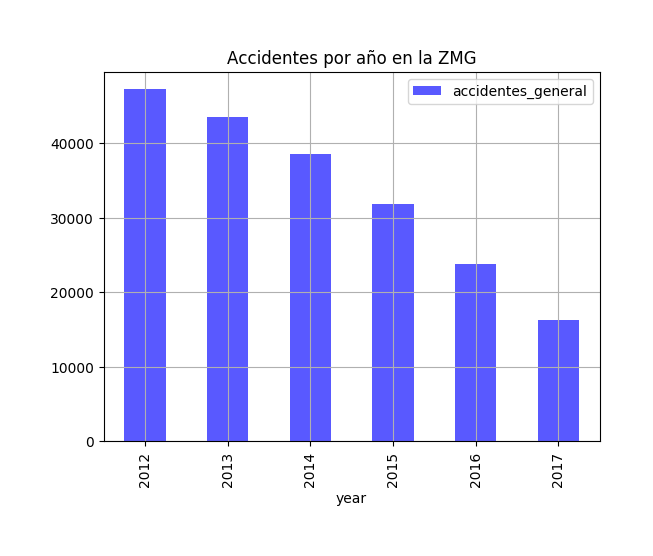
\includegraphics[width=0.60\textwidth]{resources/img/accidentes_general_img.png}
	\caption{\label{fig:accidentes_general_img} Número de accidentes viales por año dentro de la zona metropolitana de Guadalajara. Fuente: adaptación de datos de SEMOV.}
    \end{figure}

Estas políticas muestran un rendimiento excepcional en la reducción de muertes ocasionados por consumo de bebidas alcoholicas,
en donde el efecto más significativo se puede apreciar en el último año de la serie de tiempo.


	\begin{figure}[H]\centering
	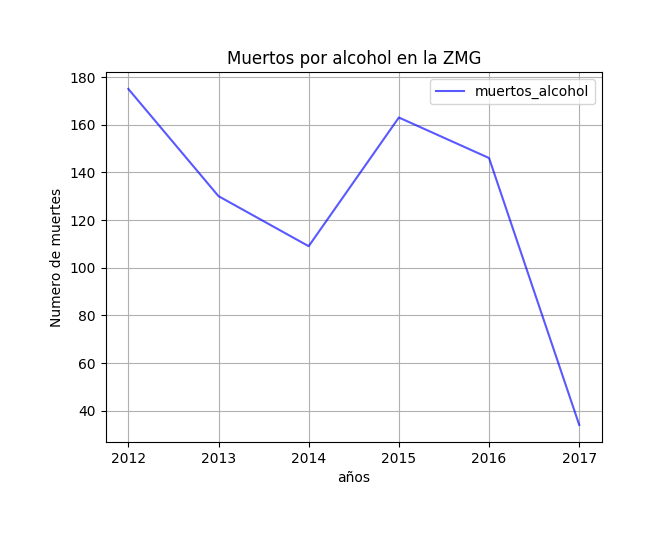
\includegraphics[width=0.60\textwidth]{resources/img/muertos_alcohol_img.png}
	\caption{\label{fig:muertes_img} Número de muertes por consumo de bebidas alcohólicas dentro de la zona metropolitana de Guadalajara. Fuente: adaptación de datos de SEMOV.}
    \end{figure}


Al analizar otras variables, es posible detectar que en general la tendencia ha sido negativa.
En particular, es de especial interés mostrar la evolución del numero de accidentes por las
categorías de lesionados involucrados, muertes total, y muertes en lugar de accidente.

	\begin{figure}[H]\centering
	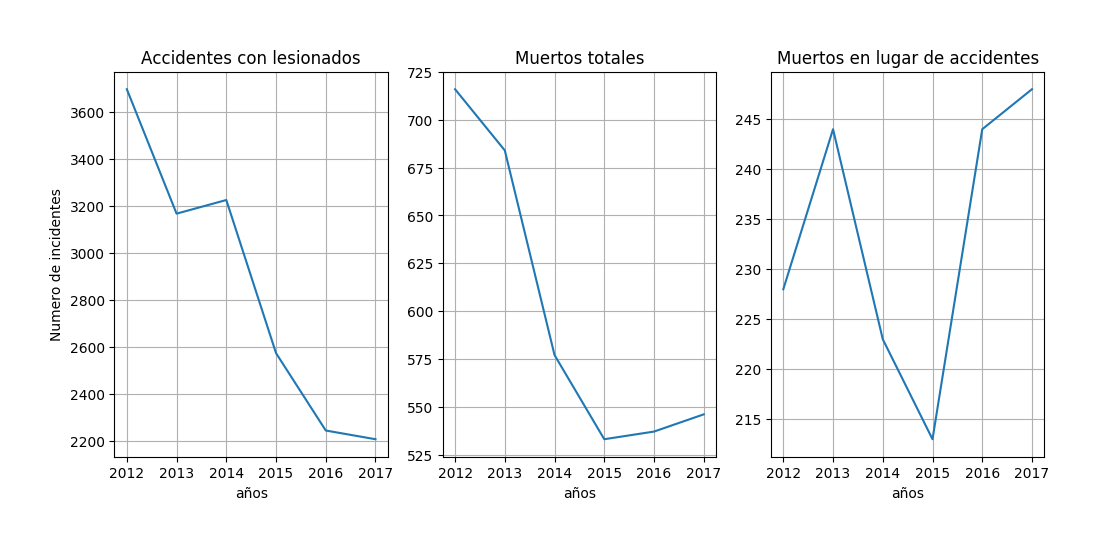
\includegraphics[width=1\textwidth]{resources/img/accidentes_general_segregacion_img.png}
	\caption{\label{fig:accidentes_general_segregacion_img} Segregación de accidentes viales dentro de la ZMG por lesionados, muertos y muertos en el lugar de accidente. Fuente: adaptación de datos de SEMOV.}
    \end{figure}

Aunque el número total de accidentes ha disminuido en forma significativa,
no todos los niveles de segregación que lo conforman presentan una disminución.
Adquiere relevancia identificar en qué segmentos la actual política de SEMOV presenta
resultados deseables y aquellos cuya situación es inmune a estas.
En este caso, se puede observar que el número de muertes en el lugar del accidente
vial ha incrementado de forma alarmante. Las causas de esto pueden variar desde
velocidad de reacción de servicios médicos, condiciones del impacto, muerte instantánea,
etc.

Una auditoria sobre la seguridad vial en la ZMG realizada por la SEMOV en colaboración con la Universidad de Guadalajara
identifican que entre los problemas de seguridad relevantes se encuentran:

	\begin{itemize}
		\item Desgaste natural del balizamiento.
		\item Falta de señales viales o en mal estado.
		\item Insuficientes espacios destinados a la circulación peatonal.
	\end{itemize}

Por otra parte, la SEMOV en su reporte "Zonas de Riesgo" clasifica las causas de accidente viales en:

	\begin{itemize}
		\item Falta de distancia de seguridad.
		\item Invadir carril contrario.
		\item Virar indebidamente.
		\item No respetar señalamiento.
		\item No respetar semáforos.
		\item Exceder límites de velocidad.
		\item Rebaso indebido.
		\item Falla mecánica del vehículo.
		\item Exceso de carga o dimensiones.
		\item Circular en sentido contrario.
		\item Falta de señalamiento.
		\item Dormitar.
	\end{itemize}


Este estudio propone el siguiente árbol de problemas (véase Figura \ref{fig:arbol}) con el fin de identificar las causas y consecuencias que desencadena el tema del presente de forma precisa.


	\begin{figure}[H]\centering
	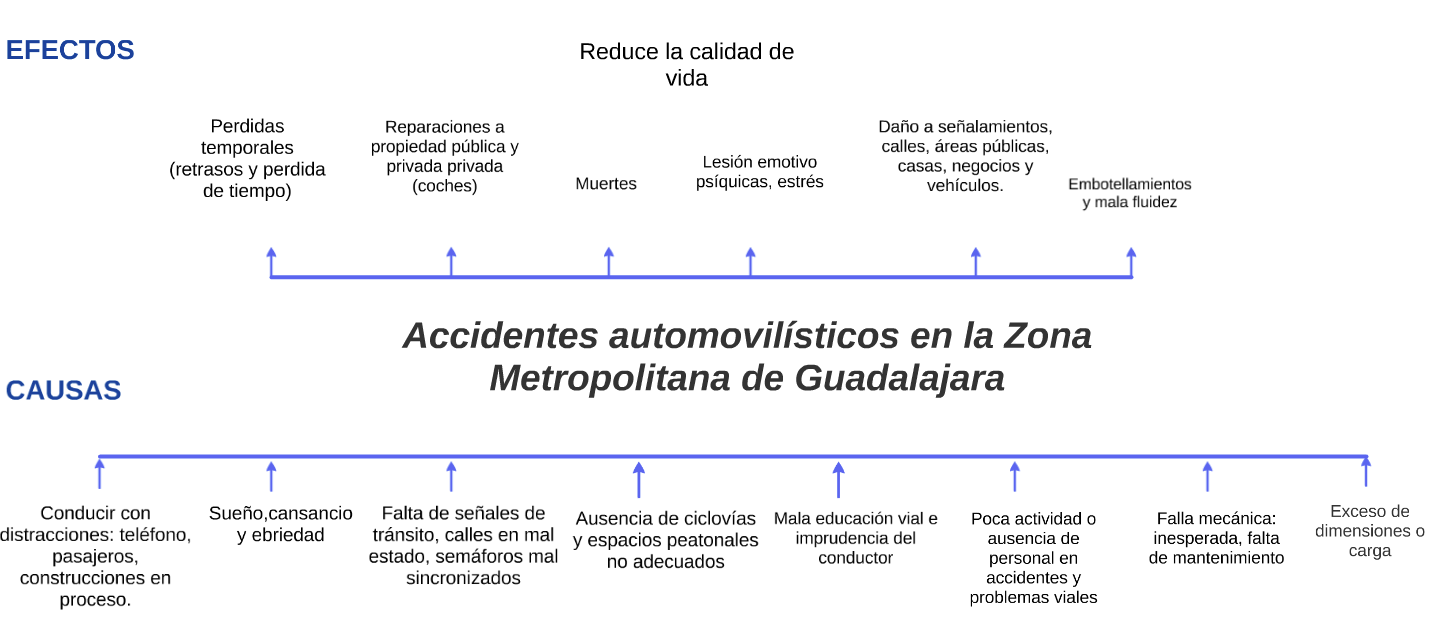
\includegraphics[width=1\textwidth]{resources/img/arbol_de_problemas.png}
	\caption{\label{fig:arbol} Árbol de problemas. Fuente: Elaboración propia.}
    \end{figure}

Las consecuencias que conlleva el problema de los accidentes automovilísticos en una zona tan transitada como lo es la Zona Metropolitana de Guadalajara van desde, daños menores como podrían ser los embotellamientos que impiden la fluidez vehicular y que a su vez ocasionan pérdidas menores temporales como son los retrasos y las pérdidas de tiempo de los conductores, lesiones emotivo-psíquicas y estrés, daños a los señalamientos, calles, áreas públicas o bien lleva a daños aún más graves como lo es la muerte. Efectos que llevan a la población a una disminución de su calidad de vida.

\newpage
\section{Objetivos del proyecto}\label{sec:objs}

En esta sección se plantean los objetivos del proyecto usando como base el
árbol de problemas (figura \ref{fig:arbol}). La intención en usar este árbol para generar
de forma análoga un árbol de objetivos. Esta metodología nos permite garantizar que
el planteamiento de los objetivos y soluciones está completamente alineado a la identificación
de los problemas. 

	\begin{figure}[H]\centering
	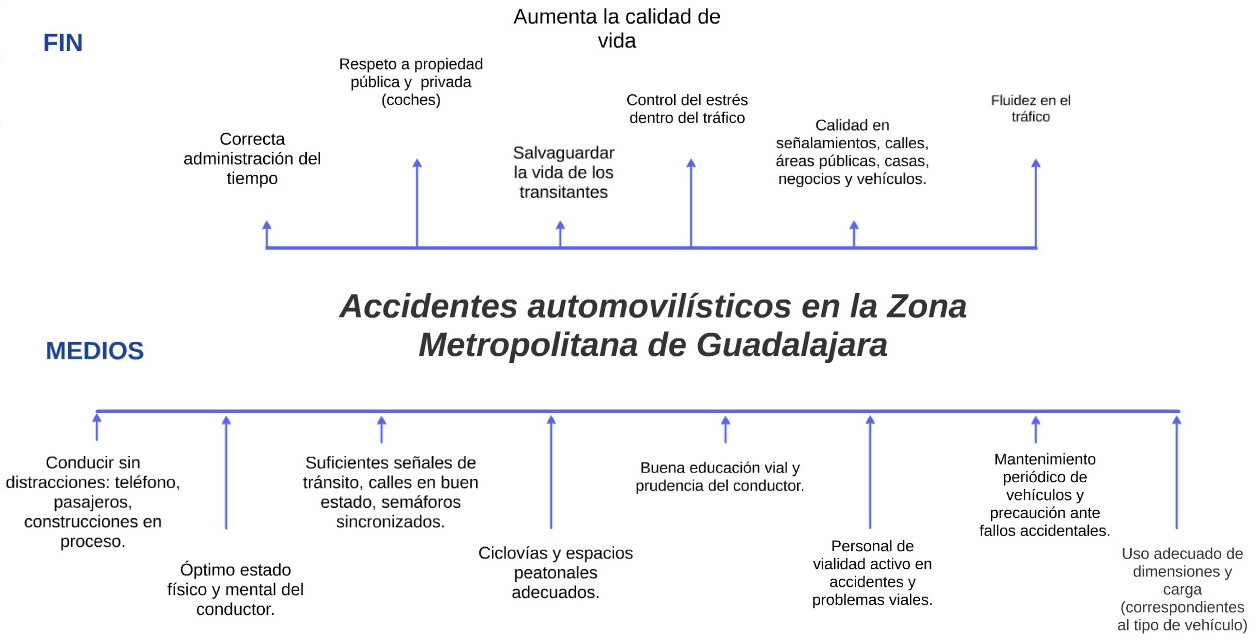
\includegraphics[width=1\textwidth]{resources/img/arbol_de_objetivos.png}
	\caption{\label{fig:arbol_obj} Árbol de objetivos. Fuente: Elaboración propia}
    \end{figure}


\subsection{Objetivo general}\label{subsec:general-objs}

Usando como referencia el árbol de objetivos (figura \ref{fig:arbol_obj}) presentado anteriormente, se propone el siguiente objetivo general:

\forceindent \textit{Mejorar la calidad de vida de los ciudadanos a través de la disminución de accidentes automovilísticos letales en la
Zona Metropolitana de Guadalajara.}

El componente medular de este objetivo reconoce que parte del bienestar social es afectado directamente por los accidentes automovilísticos. Este problema tiene el potencial de agravarse sustancialmente con el crecimiento urbano de la ZMG si no se toman las medidas y políticas adecuadas. En este sentido, se pretende analizar información pública disponible para encontrar la relación entre los accidentes viales y las acciones que se pueden llevar a cabo de forma preventiva. Entre estas acciones se identifican políticas públicas y programas sociales con la intención de generar un impacto positivo y benéfico para la sociedad. 

Actualmente se tiene evidencia de casos de éxito respecto a programas sociales que pretenden reducir los accidentes viales de una causa en particular. Dentro de estos casos, destaca el programa de "Salvando Vidas", coordinado por la Secretaría de Movilidad, en donde se atiende de forma exclusiva el consumo de alcohol indebido por conductores de vehículos.

\subsection{Objetivo específico}\label{subsec:specific-objs}

Se propone el siguiente objetivo específico:

\forceindent \textit{Disminuir el número de accidentes automovilísticos letales en la Zona Metropolitana de Guadalajara mediante un esquema de incentivos orientado al uso apropiado del celular.}

Este objetivo se deriva directamente de la parte inferior del árbol en la figura \ref{fig:arbol_obj}. La intención es atender de forma particular y precisa una de las causas más relevantes de la problemática. Esto con el afán de generar un impacto de alto grado y contribuir de una forma más significativa al objetivo general. En particular, se seleccionó este objetivo específico puesto que el uso inadecuado de tecnología celular en zonas urbanas ha presentado una tendencia alcista alarmante.


\newpage
\section{Análisis de los participantes}\label{sec:participants}

El alcance de este documento se limita a la Zona Metropolitana de Guadalajara. Tal zona está integrada por varios municipios, los cuales conforman el área urbana en su conjunto y comparten infraestructura relevante. Los incidentes viales afectan a la "zona urbana" de forma agregada; por esta razón la problemática a tratar trasciende al orden de gobierno municipal. En este sentido, el siguiente orden de gobierno inmediato es el Estado de Jalisco, en el cual se identifican varios participantes. Por otra parte, la naturaleza del problema tiene una orientación publica significativa. En este caso los ciudadanos pertenecientes a la ZMG están involucrados de forma directa. 

En la siguiente tabla se desglosan los participantes:

\begin{table}[H]\centering
\begin{tabular}{l r}
\hline
Participantes & Competencia \\
\hline\hline
Secretaría de Movilidad & Estatal \\
Instituto de Movilidad y Transporte & Estatal \\
Secretaría de Infraestructura y Obra Pública & Estatal \\
Secretaría de Planeación y Administración Financiera & Estatal\\
Ciudadanos & Público \\

\hline
\end{tabular}
\end{table}

\subsection[SEMOV]{Secretaría de Movilidad del Estado de Jalisco}\label{subsec:semov}

La Secretaría de Movilidad (SEMOV) es la autoridad en materia de tránsito y vialidad del Estado de Jalisco. Son los encargados de la seguridad y calidad en el desplazamiento de vehículos dentro de la entidad. 

\subsection[IMTJ]{Instituto de Movilidad y Transporte del Estado de Jalisco}\label{subsec:imtj}

El Instituto de Movilidad y Transporte es un organismo público y descentralizado del Estado de Jalisco con el objetivo principal de promover la movilidad sustentable. Este instituto se encarga de proponer e implementar actividades para eficientar el transporte. Tiene la facultad de emitir opinión técnica a la SEMOV. 

\subsection[SIOP]{Secretaría de Infraestructura y Obra Pública del Estado de Jalisco}\label{subsec:siop}

La Secretaría de Infraestructura y Obra Pública (SIOP) se encarga del desarrollo, proyección y construcción de obras públicas en el Estado de Jalisco. 

\subsection[SEPAF]{Secretaría de Planeacion y Administracion Financiera de Jalisco}\label{subsec:sepaf}
La Secretaria de Planeacion y Administración Financiera (SEPAF) es responsable de garantizar que se destinen los bienes y recursos estatales a las acciones que son prioridades en la planeación y desarrollo del estado. 

\newpage

\section{Alternativas de solución}\label{sec:alternatives}
[Esta sección es la más larga y
laboriosa del proyecto. Dependiendo
del proyecto, se evaluarán 1 o 2
alternativas de solución. 
% * <rohdzmota@gmail.com> 2018-02-17T00:23:06.435Z:
% 
% Definir un indicador para el problema central y 3 indicadores para el específico.
% Considerar efectos quantificables: 
% * vidas salvadas (monetización)
% * costo promedio de siniestros (personales, infraestructuras, tiempo en embotellamiento)
% * numero de colisiones
% * indicador respecto a población afectada. 
% ^.

\subsection{Metodologías}

\subsection{Situación actual}\label{subsec:actual}

Actualmente se puede apreciar una disminución en el número de accidentes viales debido a
una política para identificar el uso y consumo ilegal de bebidas alcohólicas al conducir.
No obstante, a partir del 2015 el numero de accidentes automovolísticos letales ha comenzado
a aumentar. Esto puede ser producto de la reciente alta adopción de tecnologías celulares en la Zona
Metropolitana de Guadalajara. En el año 2015 el porcentaje de usuarios de tecnología celular en Jalisco
era del 76.32\%. Esta cifra aumentó a 81.80\% en 2016. La figura \ref{fig:tipo_celular} muestra la
proporción de celulares comúnes y smartphones.


	\begin{figure}[H]\centering
	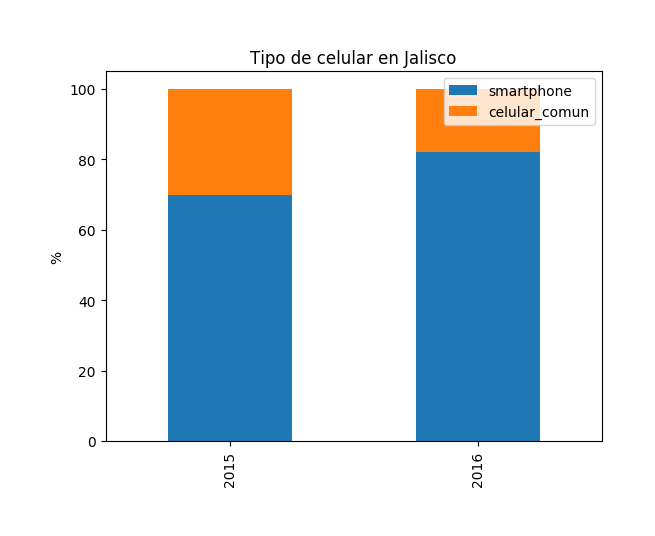
\includegraphics[width=0.6\textwidth]{resources/img/tipo_de_celular.png}
	\caption{\label{fig:tipo_celular} Crecimiento del Smartphone. Fuente: Elaboración propia}
    \end{figure}

La adopción de smartphones ha aumentado durante el periodo del 2015 al 2016 desde
el 69.8\% hasta el 82.2\%. En recientes estudios, la Organización Mundial de la Salud ha identificado
el uso del celular como un alto factor de riesgo al conducir debido a que genera distracciones
visuales, cognitivas, físicas y auditivas.

Por otra parte, la Secretaría de Movilidad identificó en 2016 el porcentage de conductores afectados
por distacciones de celular en distintos municipios pertenecientes a la Zona Metropolitana de Guadalajara.
El promedio de la Zona indica que al menos 60\% de los conductores se ven afectados por este tipo
de distracciones al conducir.

	\begin{figure}[H]\centering
	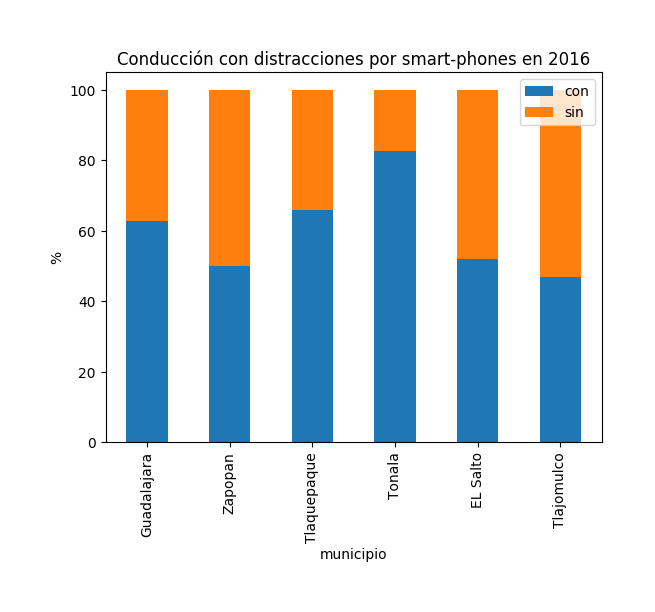
\includegraphics[width=0.6\textwidth]{resources/img/manejo_con_celular.png}
	\caption{\label{fig:tipo_celular} Uso de celular al conducir. Fuente: Elaboración propia}
    \end{figure}

Aunado a esto, el parque vehícular en el estado de Jalisco tiene una tendencia alcista. Esto significa que el número
de vehículos en circulación está en aumento. Tomando en consideración que la adopción de Smartphones
también presenta una tendencia a la alta y está fuertemente correlacionada con accidentes automovilísticos,
la seguirdad víal puede verse afectada de forma relevante.

	\begin{figure}[H]\centering
	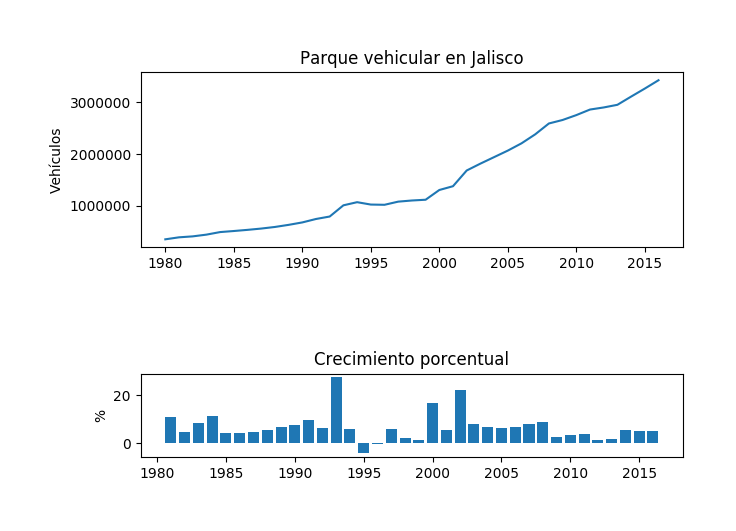
\includegraphics[width=1\textwidth]{resources/img/parque_vehicular.png}
	\caption{\label{fig:parque_vehicular} Vehículos en circulación. Fuente: Elaboración propia}
    \end{figure}

\subsubsection{Definición de indicadores}

[TODO: definir indicador para objetivo general y 3 para el objectivo específicio]]

\subsubsection{Pronósitico de la adopción de tecnología celular}

[TODO: Usar método exponencial]

\subsubsection{Pronósitico del crecimiento del parque vehicular}

[TODO: Usar cadenas de markov]


\subsection{Situación con proyecto}


\subsection{Análisis Costo-Beneficio}
% * <rohdzmota@gmail.com> 2018-02-17T00:17:19.479Z:
% 
% Beneficios - Costos > 0  -- rentable, TIR
% 
% ^.

\subsection{Simulación Montecarlo y Análisis de Sensibilidad}

\subsection{Resultados}
% * <rohdzmota@gmail.com> 2018-02-17T00:16:37.605Z:
% 
% Concluir si el proyecto es rentable o no
% 
% ^.

\newpage
\section{Elaboración de la MIR}\label{sec:mir}
[agregar contenido]

\newpage
\section{Conclusiones}\label{sec:conclutions}
[agregar contenido]

\newpage
\section{Bibliografía}\label{sec:references}
[agregar contenido]

\end{document}